%% LyX 1.6.2 created this file.  For more info, see http://www.lyx.org/.
%% Do not edit unless you really know what you are doing.
\documentclass[english]{scrartcl}
\usepackage[T1]{fontenc}
\usepackage[latin9]{inputenc}
\usepackage[letterpaper]{geometry}
\geometry{verbose,tmargin=2cm,bmargin=2cm,lmargin=2cm,rmargin=1cm,headheight=2cm,headsep=1cm,footskip=0.5cm}
\usepackage{graphicx}

\usepackage{babel}

\begin{document}

\title{Sorting Criterion for Slip and Twin system in HCP}


\author{YunJo Ro}

\maketitle
This document attempts to show how we sort the order of the slip and
twin system for Hex (or hcp) structure in lattice.f90. 


\section{Slip system }

An intersection between slip and basal plane is used in order to sort
the slip system as illustrated in Figures \ref{Fig:BasalPrismSlip}
and \ref{Fig:Pyr<a><c+a>}. Numbers in Figures \ref{Fig:BasalPrismSlip}
and \ref{Fig:Pyr<a><c+a>} indicate the sequence of each slip system
in {}``lattice.f90''. In {}``lattice.f90'', No. 4 - 6 for basal
and prism <a> slip do not include (Figure \ref{Fig:BasalPrismSlip}).
In Figure \ref{Fig:Pyr<a><c+a>}, pyramidal slip <c+a> was used two
criterions to sort the 12 slip systems; i) intersection between pyramidal
slip plane and basal plnae, and ii) <a> direction. 

%
\begin{figure}[tbph]
\begin{centering}
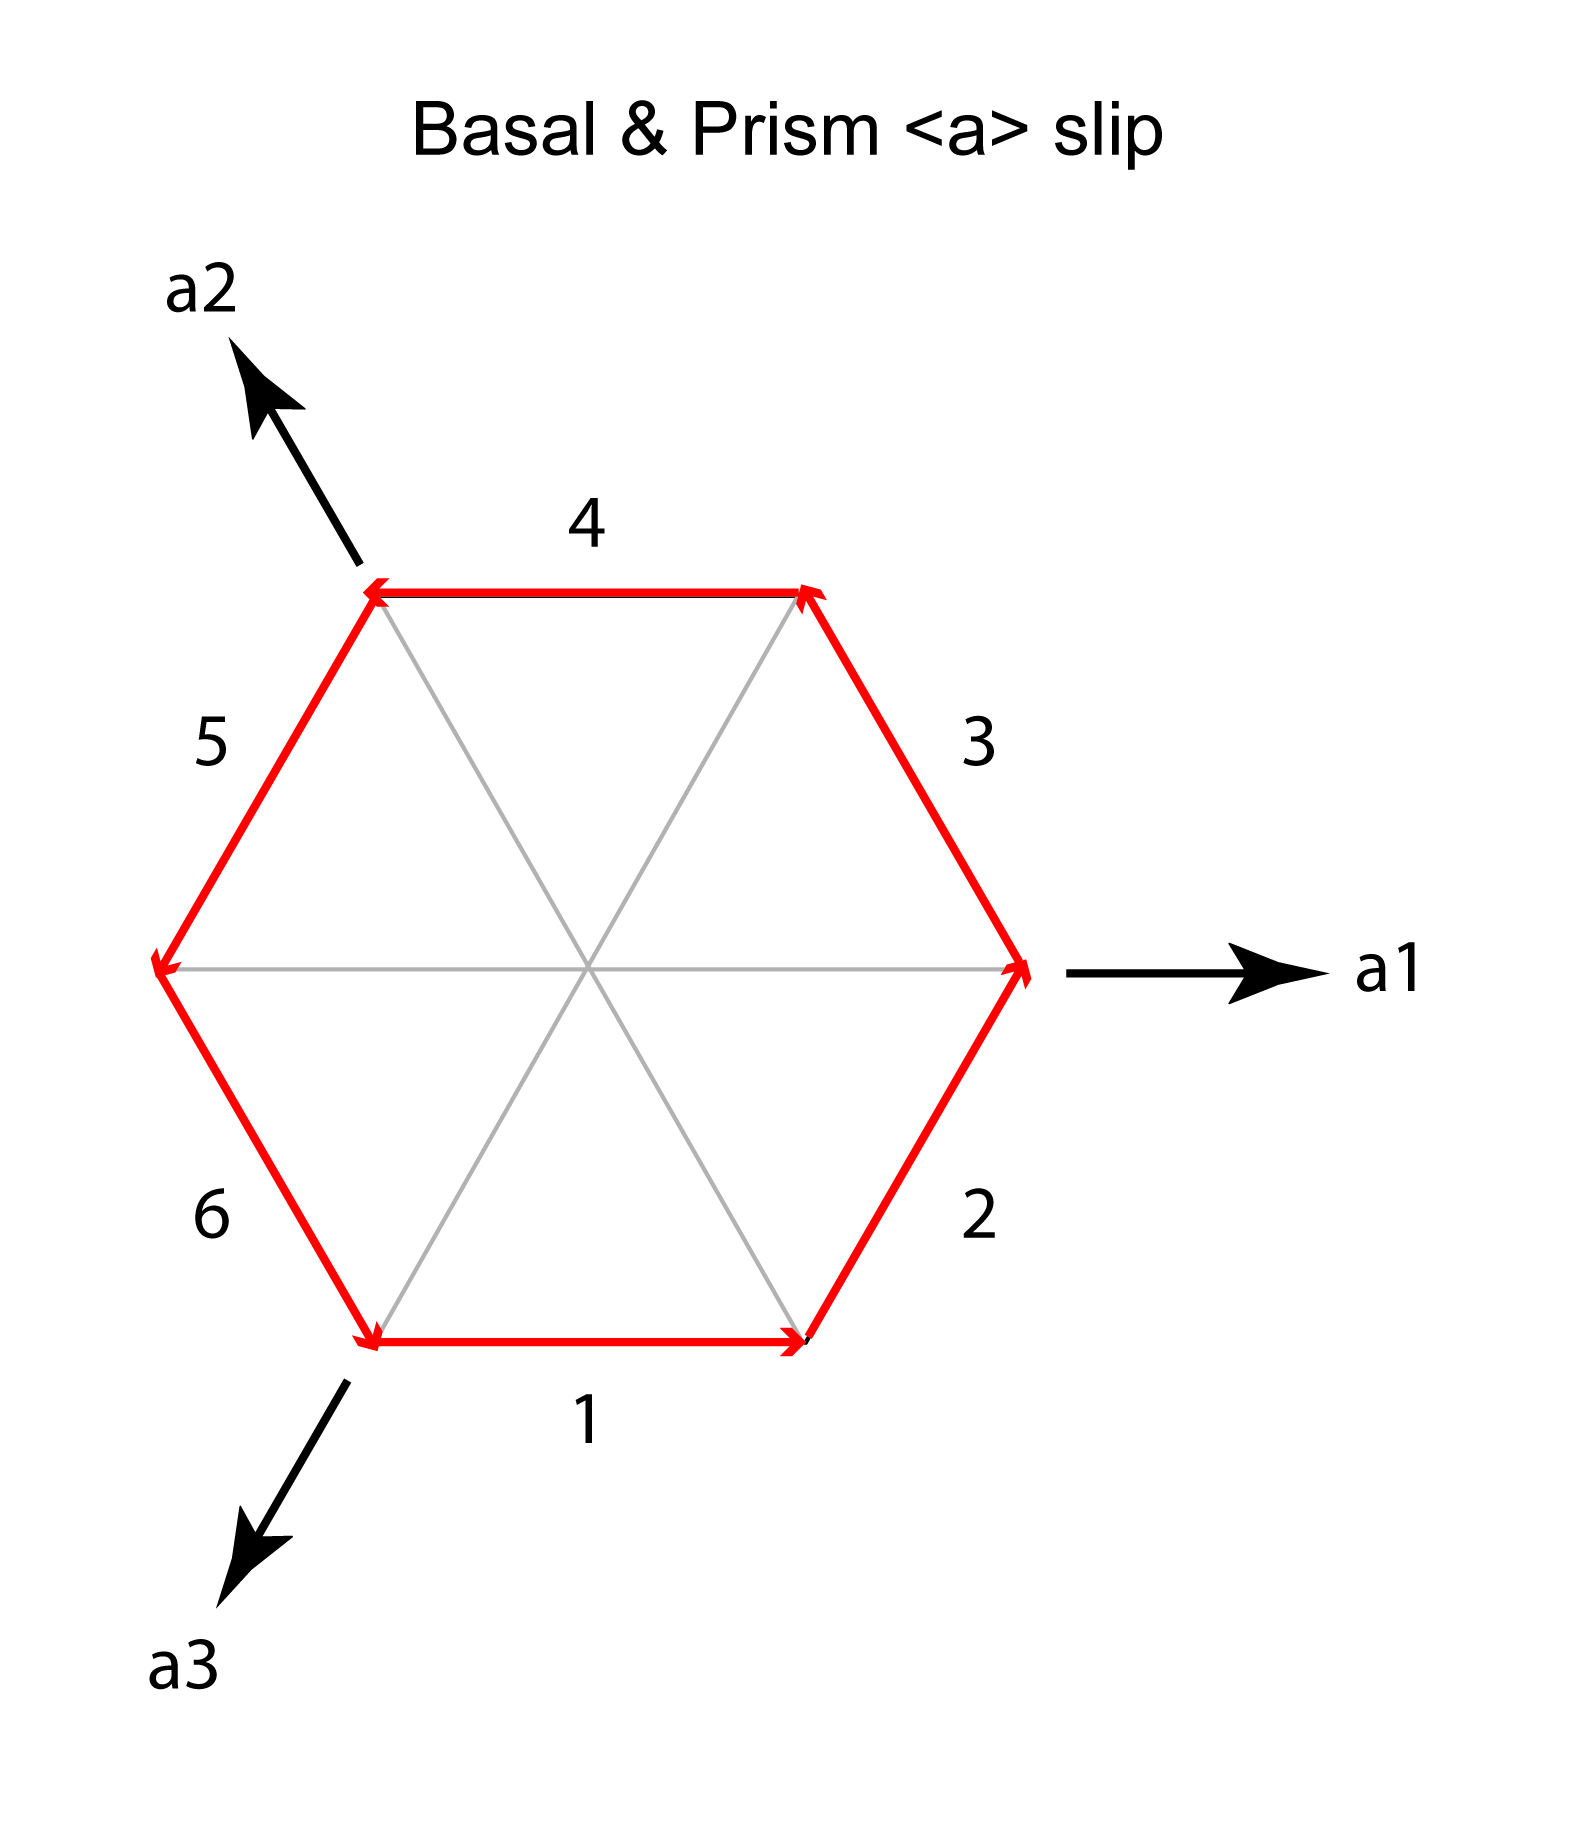
\includegraphics[clip,scale=0.18]{figures/slipSystemForHCP}\caption{Basal and prism <a> slip.}
\label{Fig:BasalPrismSlip}
\par\end{centering}


\end{figure}
%
\begin{figure}[tbph]
\centering{}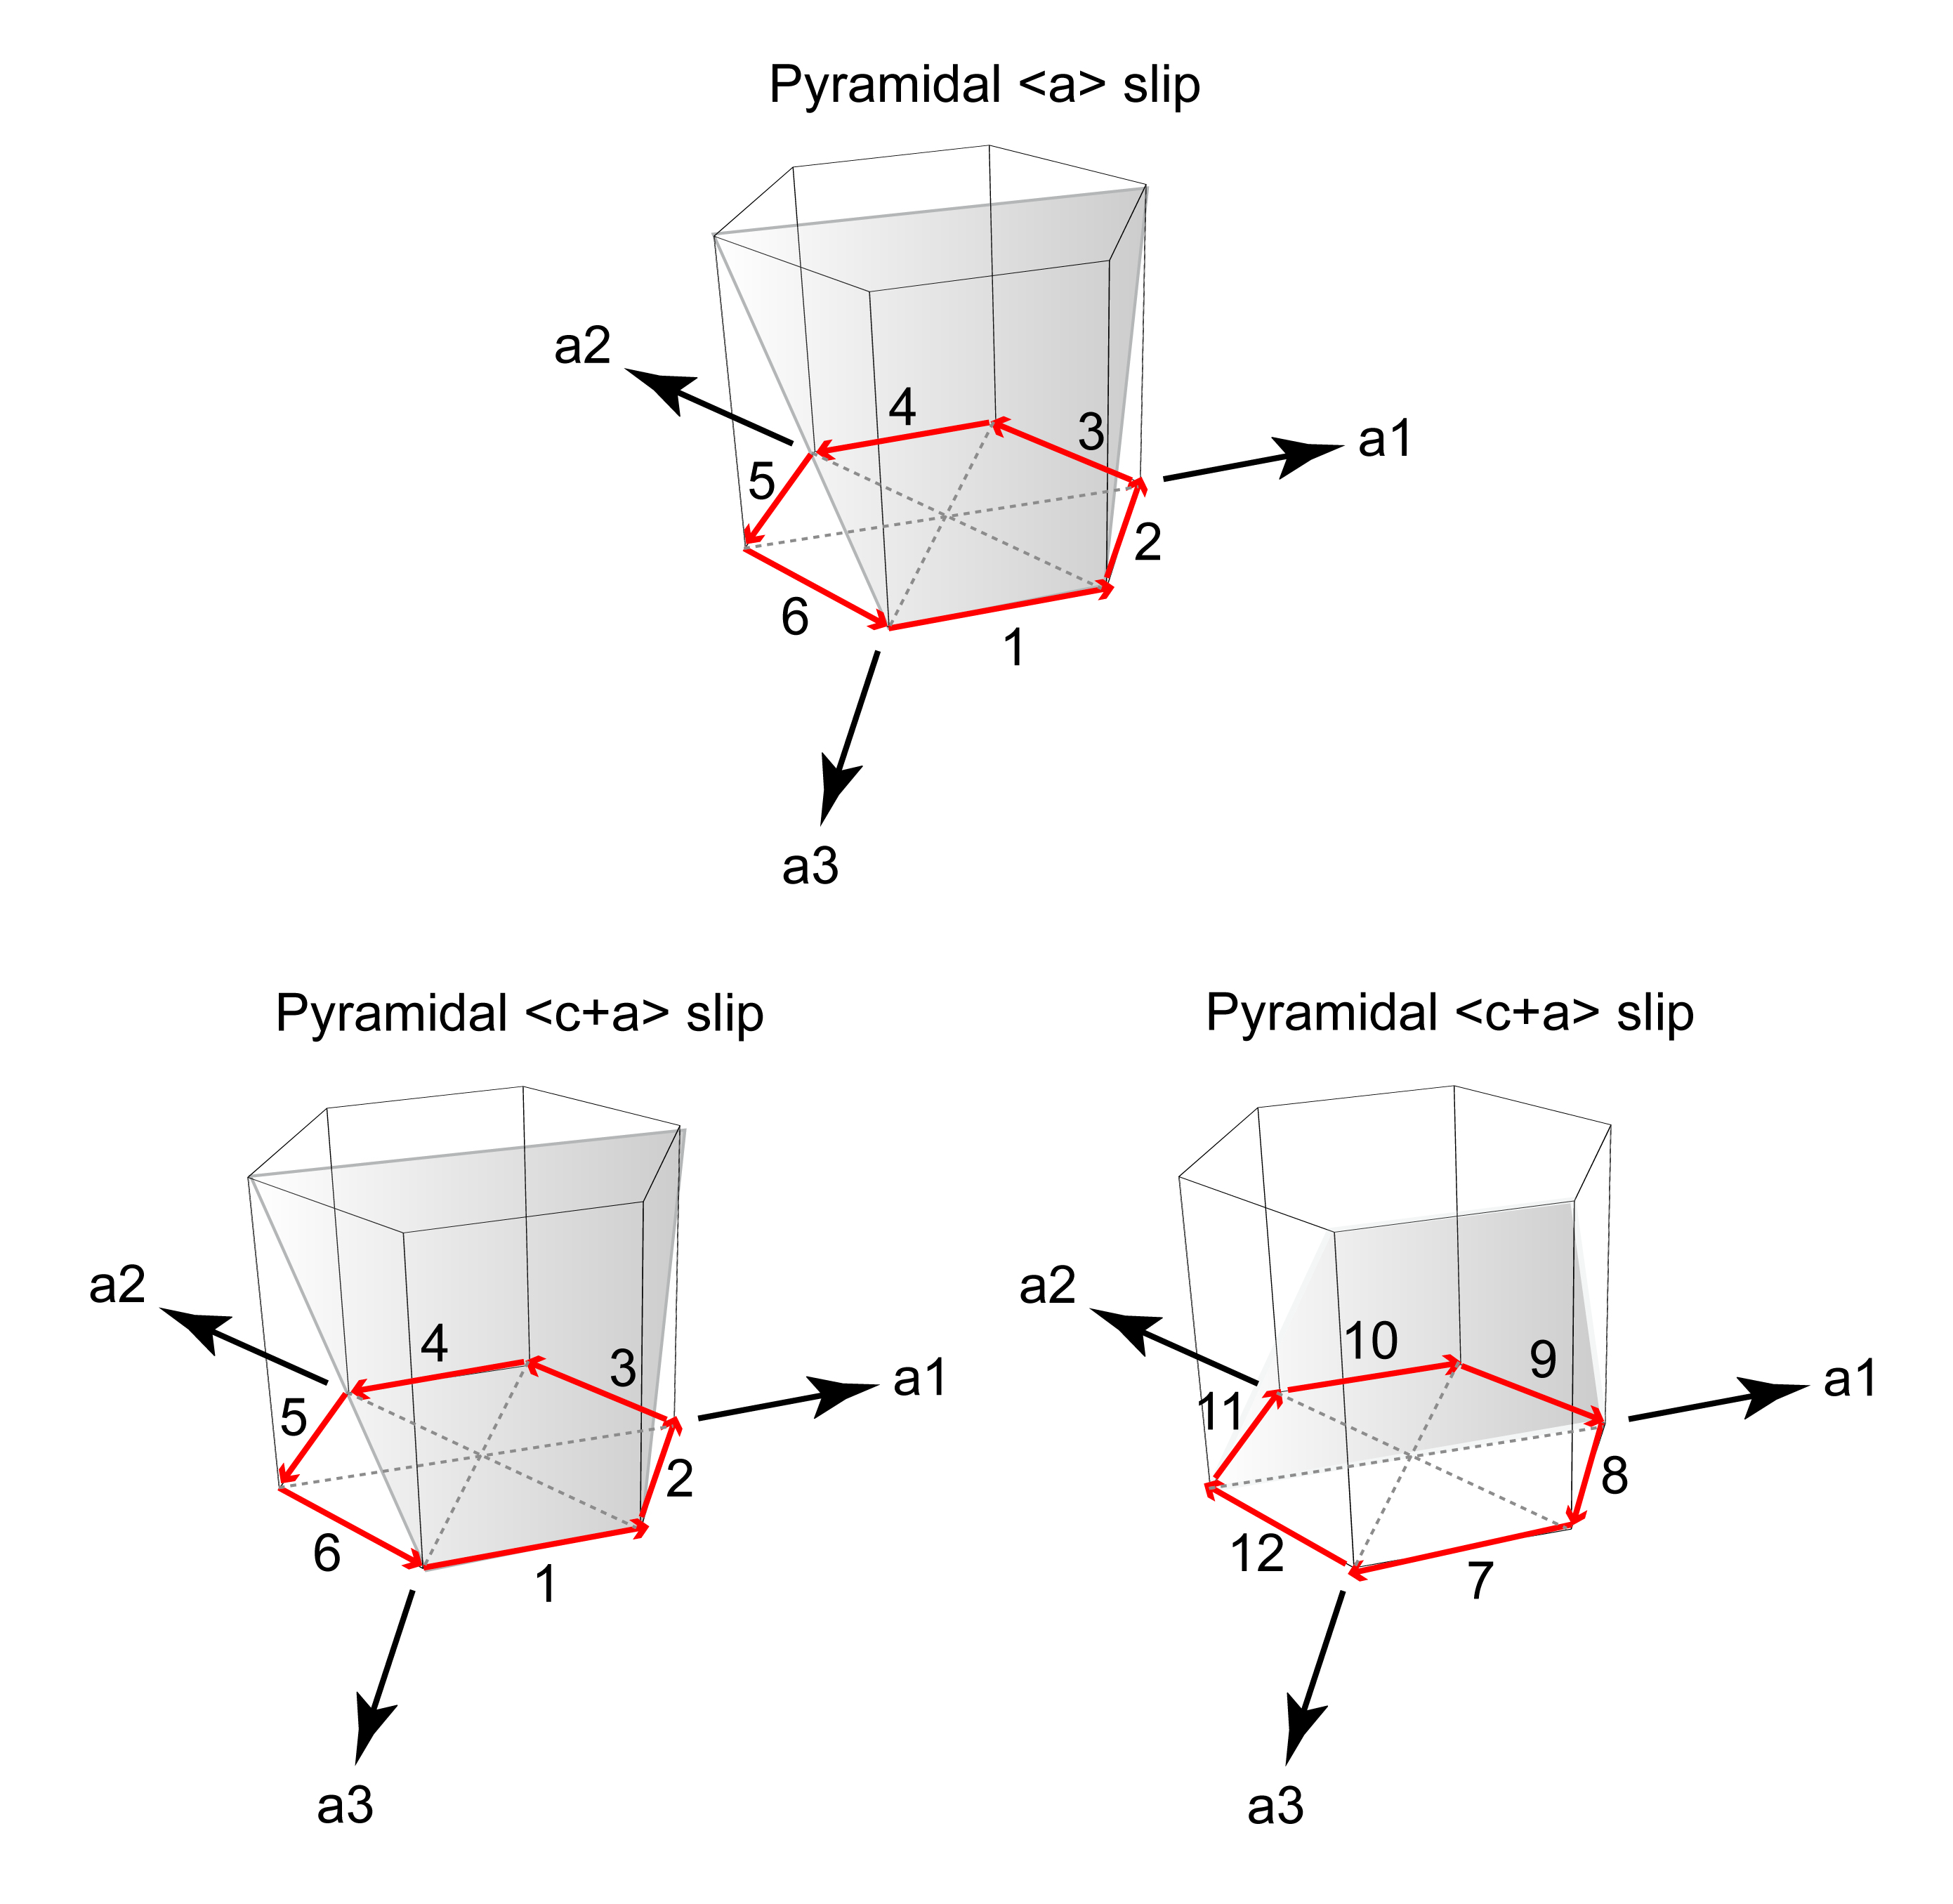
\includegraphics[clip,scale=0.18]{figures/slipSystemForHCP-pyr}\caption{Pyramical <a> and <c+a> slip.}
\label{Fig:Pyr<a><c+a>}
\end{figure}


\clearpage{}


\section{Twin system}

An intersection between twin and basal plane is used in order to sort
the twin system as illustrated in Figures \ref{Fig:TwinType1} and
\ref{Fig:TwinType2}. Numbers in Figures \ref{Fig:TwinType1} and
\ref{Fig:TwinType2} indicate the sequence of each twin system in
{}``lattice.f90''.

%
\begin{figure}[tbph]
\centering{}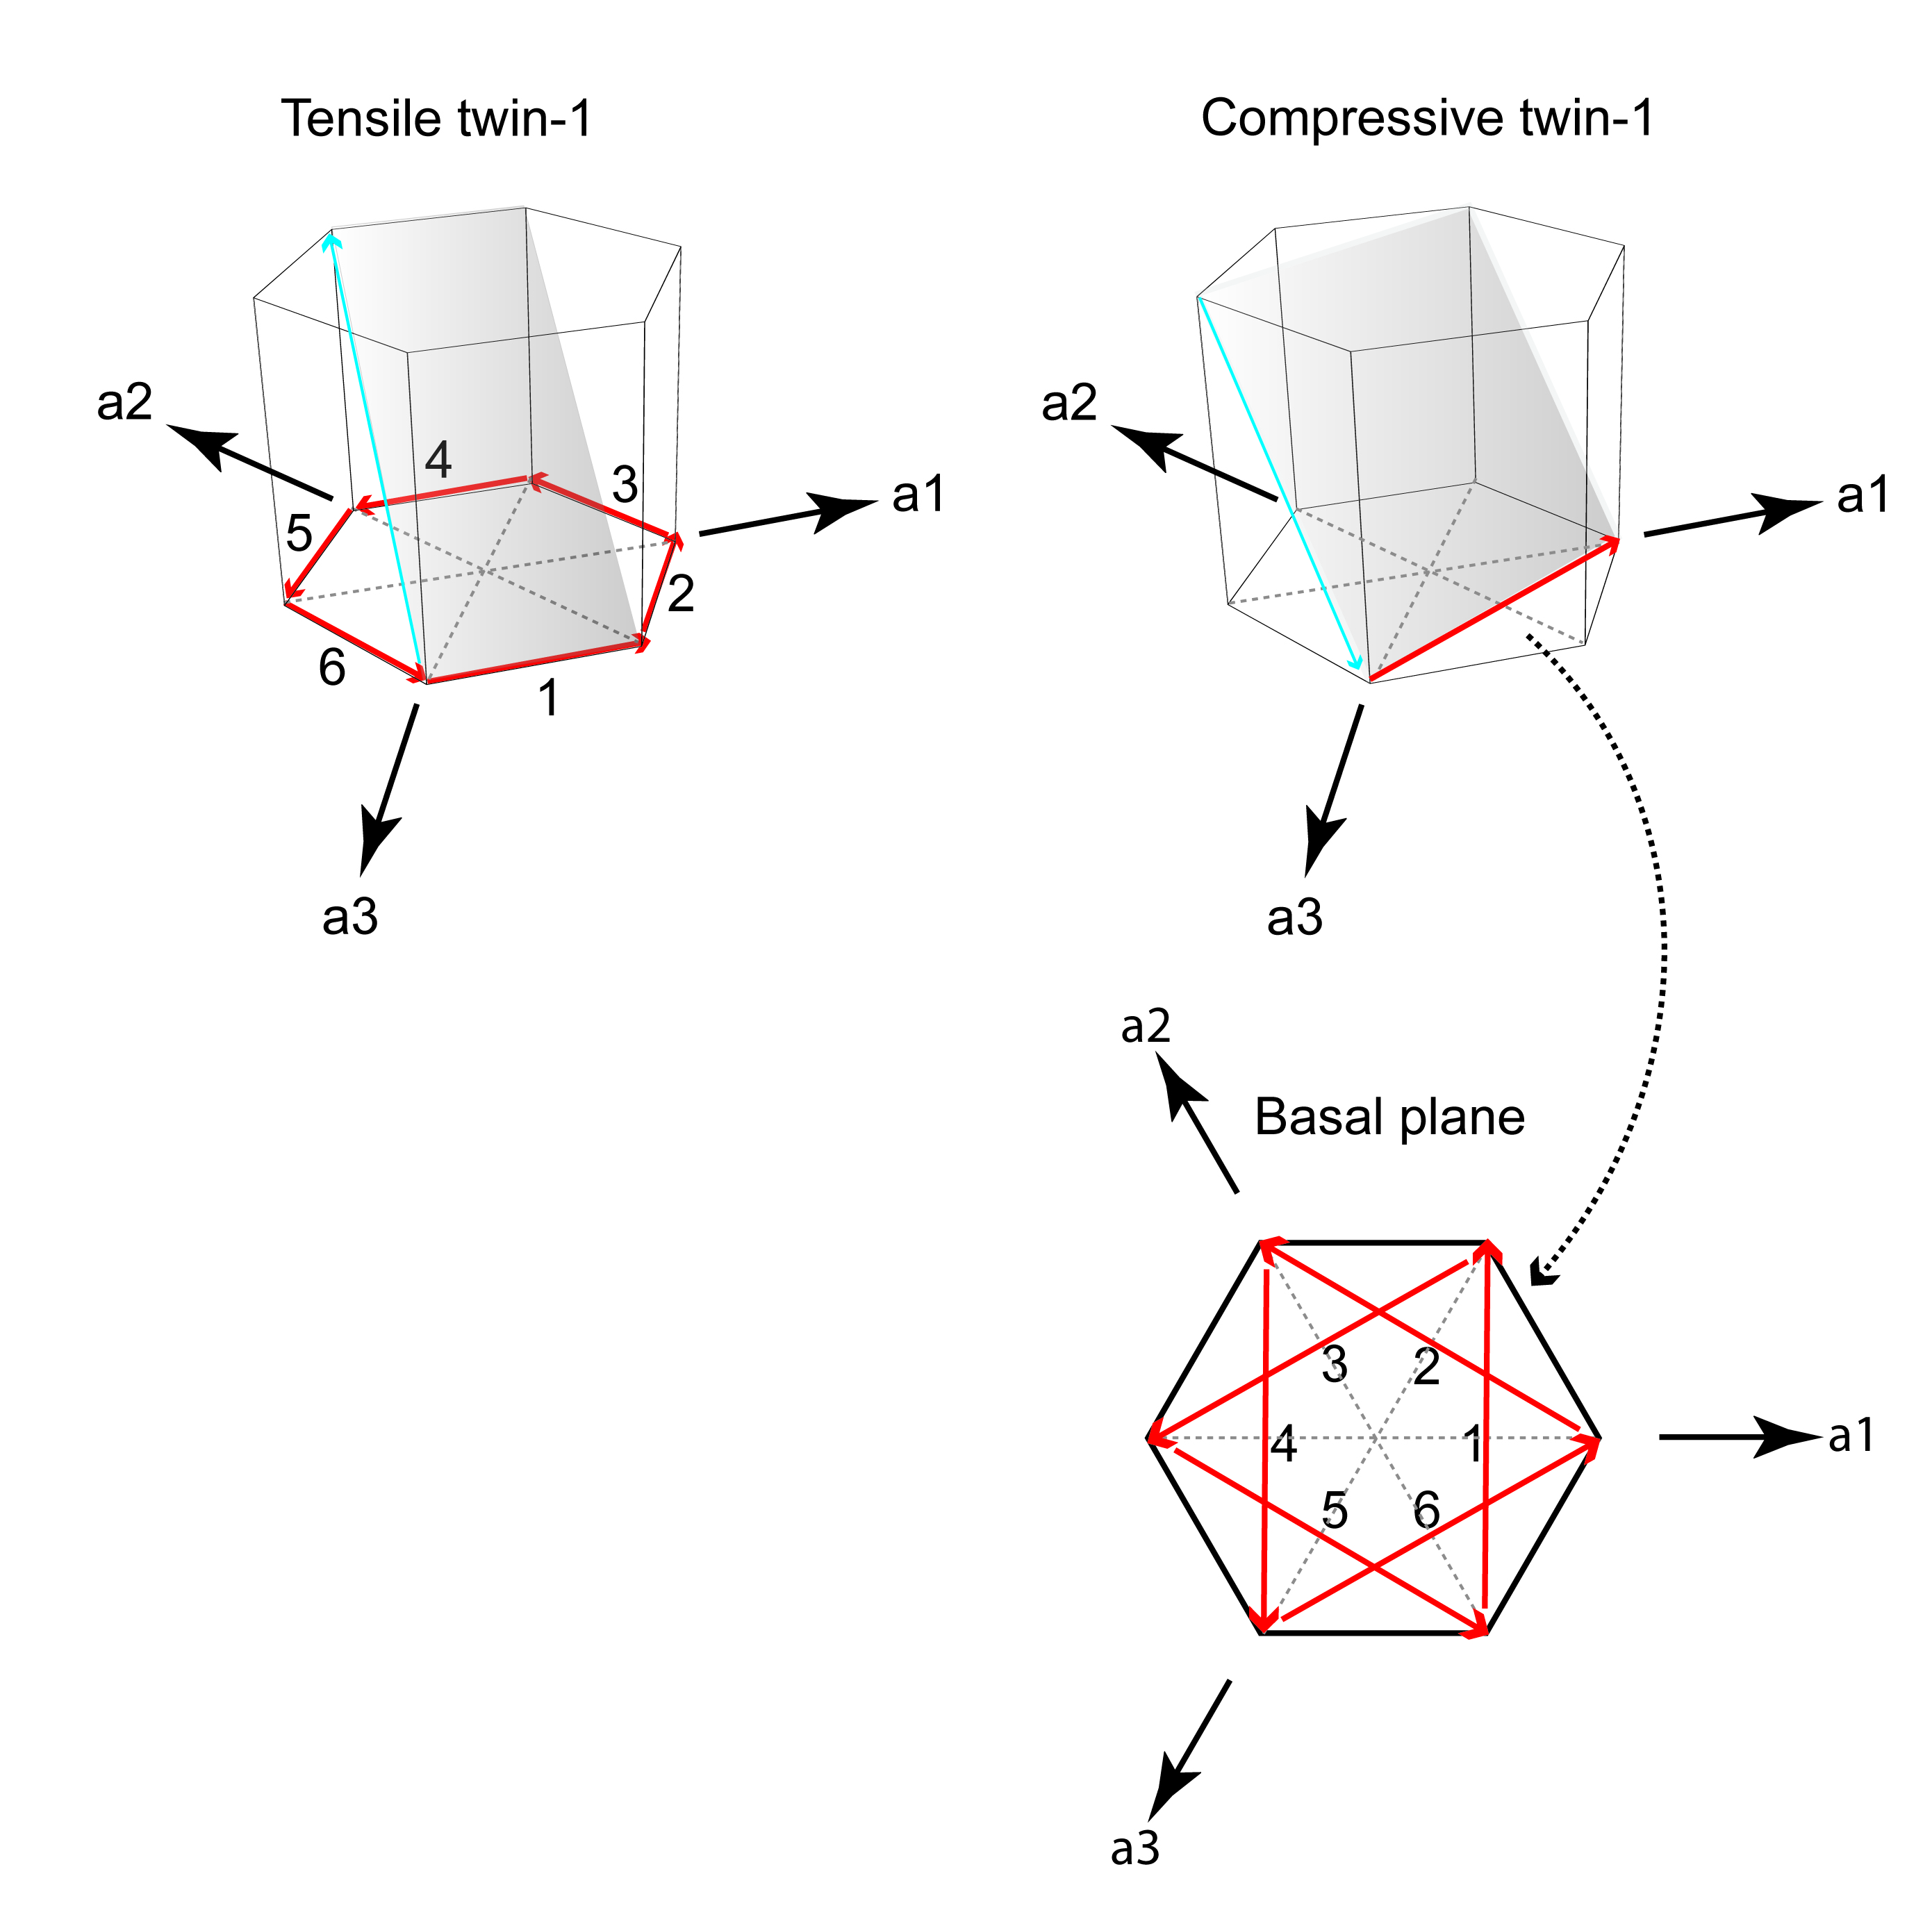
\includegraphics[clip,scale=0.18]{figures/twinSystemForHCP-1}\caption{Tensile and compressive twin type 1}
\label{Fig:TwinType1}
\end{figure}
%
\begin{figure}[tbph]
\centering{}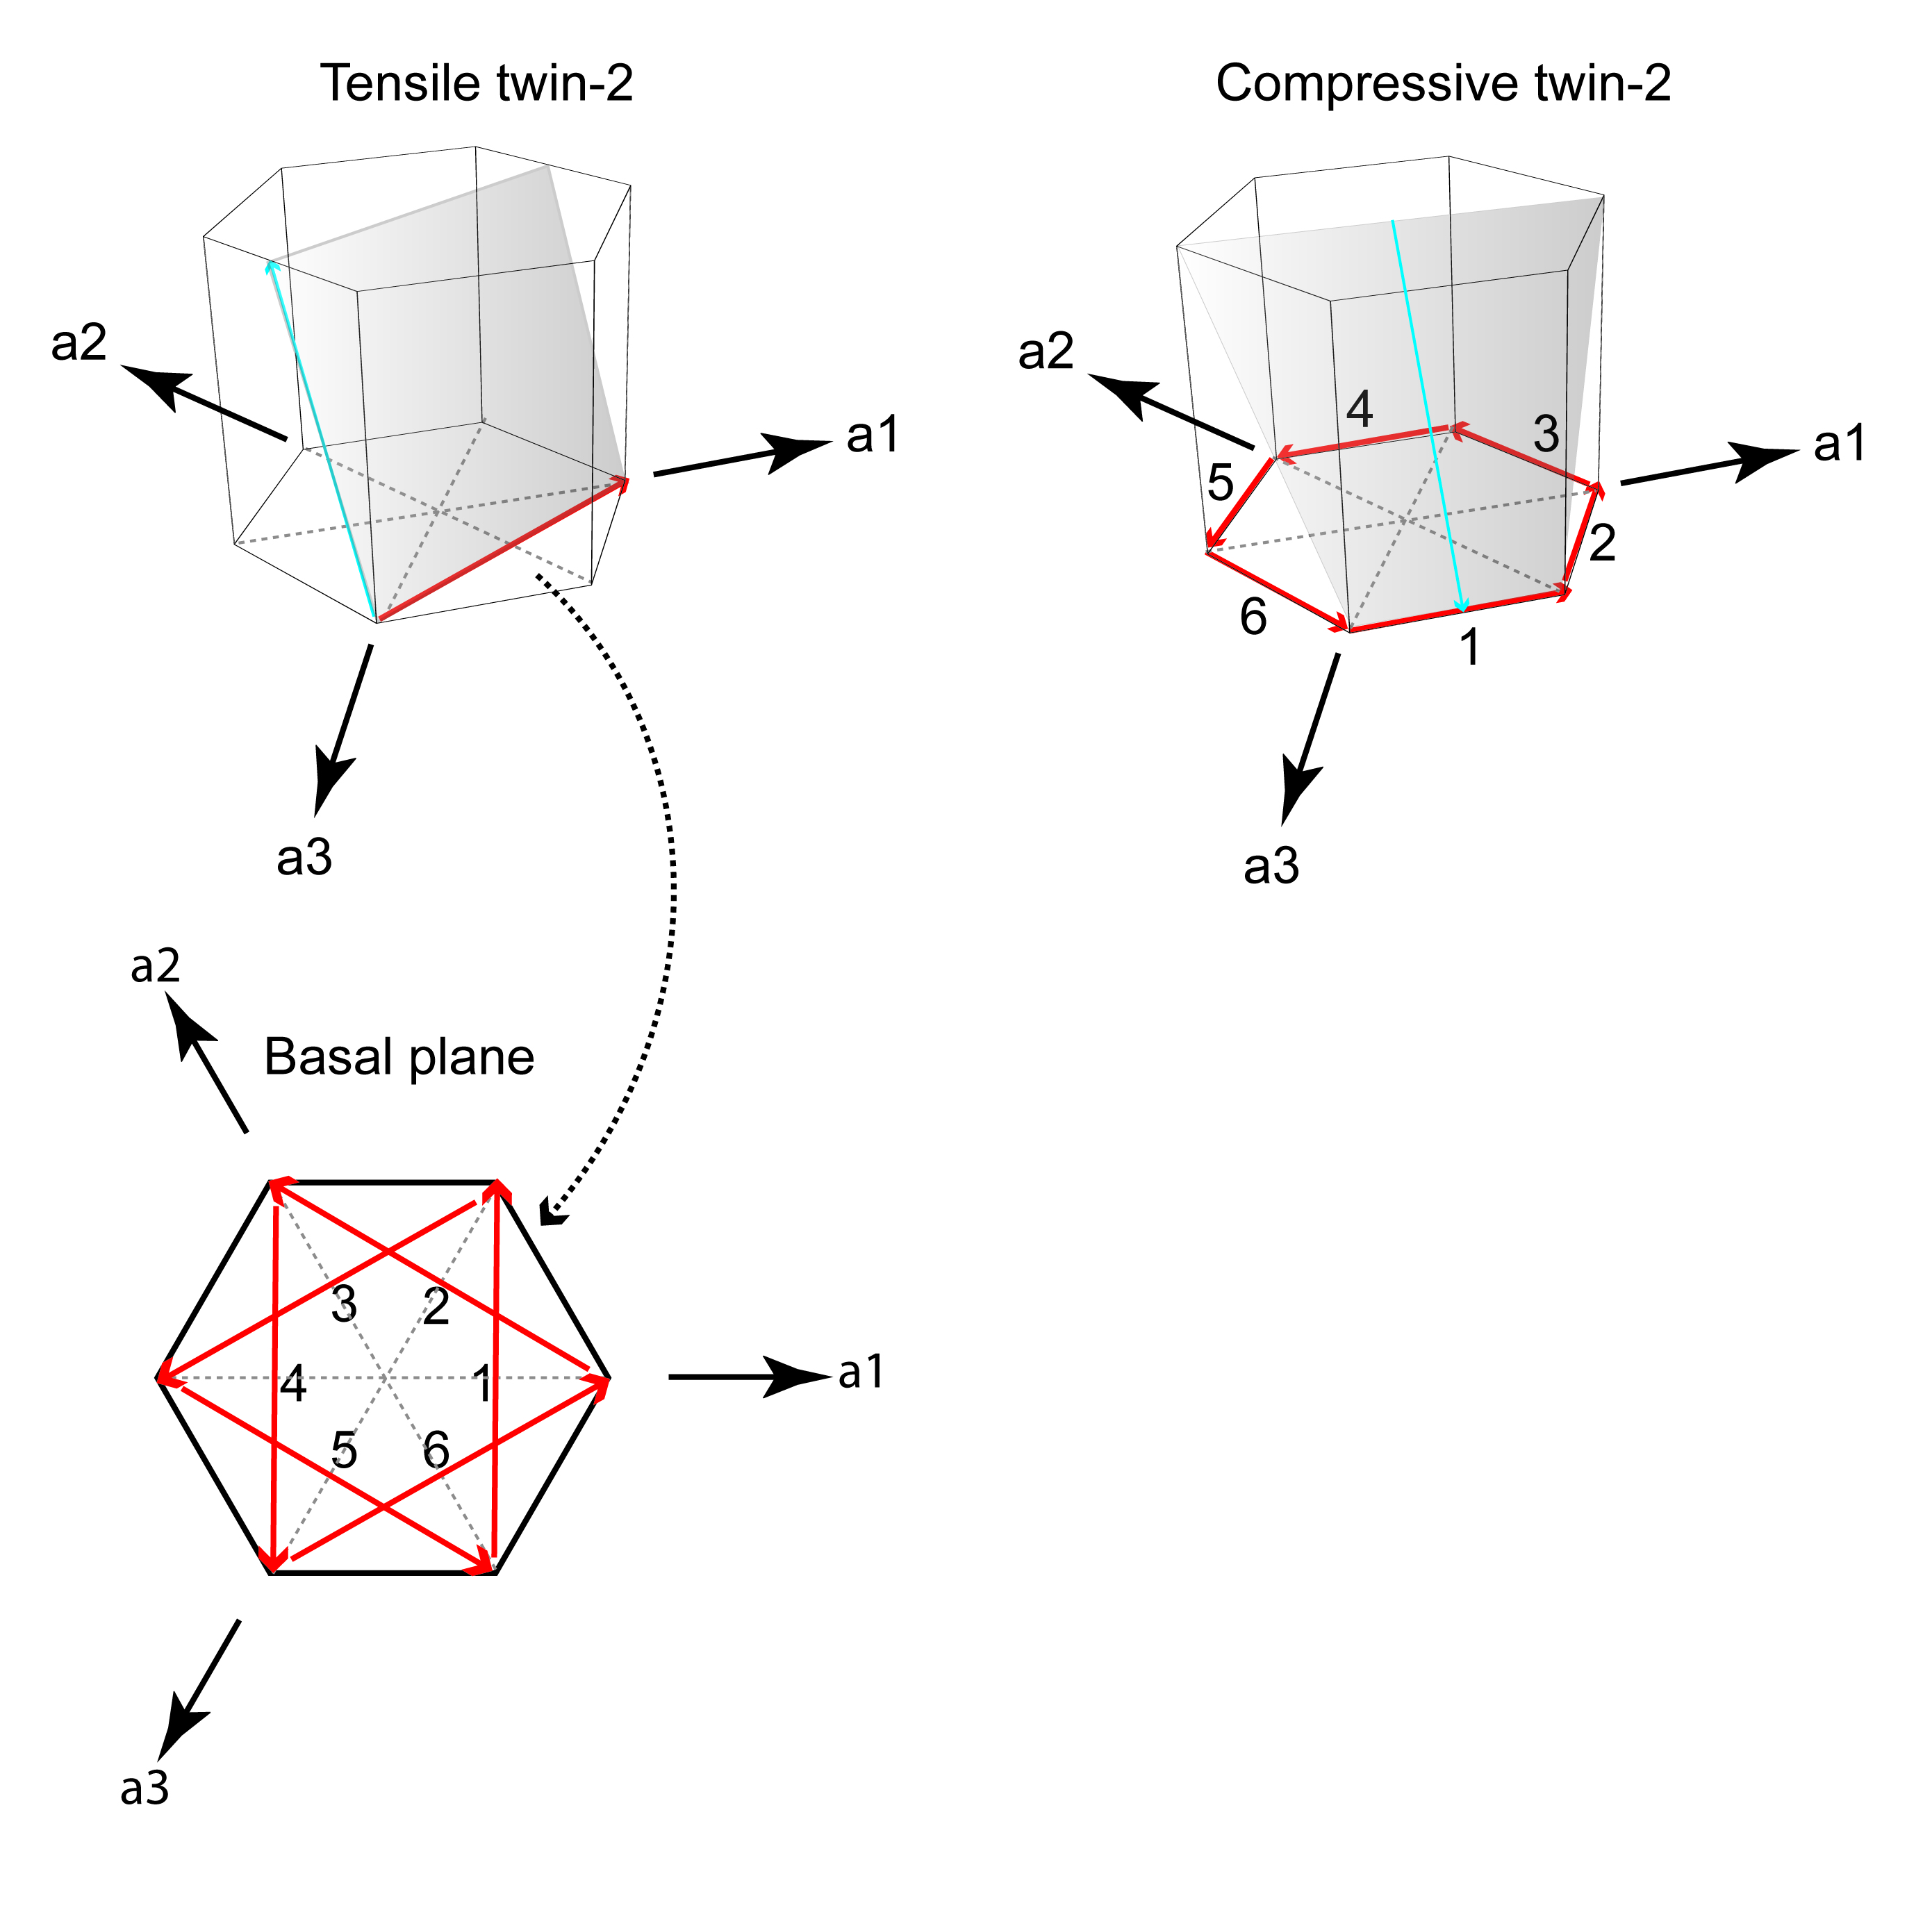
\includegraphics[clip,scale=0.18]{figures/twinSystemForHCP-2}\caption{Tensile and compressive twin type 2}
\label{Fig:TwinType2}
\end{figure}

\end{document}
